% Restored from the original manuscript, without introducing new author claims.
\begin{IEEEbiography}[{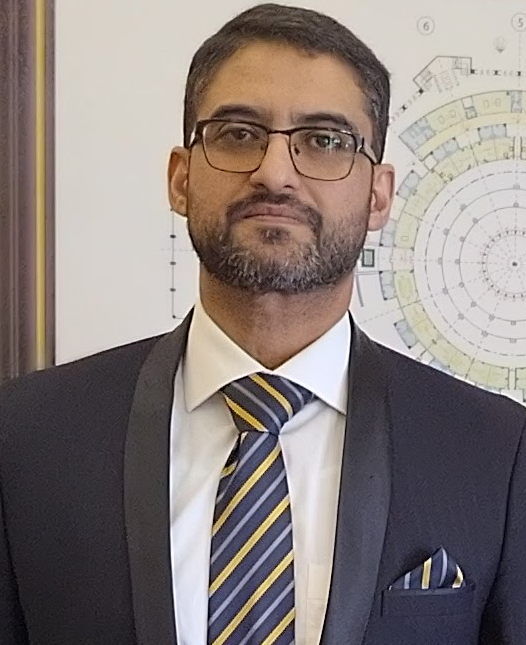
\includegraphics[width=1in,height=1.25in,clip,keepaspectratio]{figures/umair_original_portrait.png}}]{Muhammad Umair Raza}
received the B.E. degree in avionics engineering from NUST, Pakistan, in 2008. He completed his M.S. studies in avionics engineering (signal and image processing) at Air University, Islamabad, in 2015; the degree was conferred in 2017. He is with the Department of Avionics Engineering, College of Aeronautical Engineering, NUST, Risalpur, Pakistan. His work includes signal processing and sensing systems.
\end{IEEEbiography}
\begin{IEEEbiographynophoto}{Sohail Ahmed}
received a degree in avionics engineering from the College of Aeronautical Engineering, Pakistan, the M.S. degree in telecommunications engineering from NUST, Pakistan, and the Ph.D. degree from the University of Southampton, UK. He is a Senior Application Engineer with MathWorks, USA. His research includes communications and radar signal processing.
\end{IEEEbiographynophoto}
\begin{IEEEbiographynophoto}{Ammad Ahmed}
studied aeronautical engineering (avionics) at the National University of Sciences and Technology, Pakistan. He is an RF Engineer with NDMA, Pakistan.
\end{IEEEbiographynophoto}

% Affiliation-only factual entries; education/research details require authors.
\begin{IEEEbiographynophoto}{M. Atif Shahzad}
is with the Department of Avionics Engineering, College of Aeronautical Engineering, National University of Sciences and Technology, Risalpur, Pakistan.
\end{IEEEbiographynophoto}
\begin{IEEEbiographynophoto}{Syed M. Kazam Abbas Kazmi}
is with the Department of Avionics Engineering, College of Aeronautical Engineering, National University of Sciences and Technology, Risalpur, Pakistan.
\end{IEEEbiographynophoto}
